\subsection{Structure du premier étage}
\label{subsec:premier_etage}

\begin{figure}[h]
    \centering
    \begin{tikzpicture}
    
        \node at (0, 0) {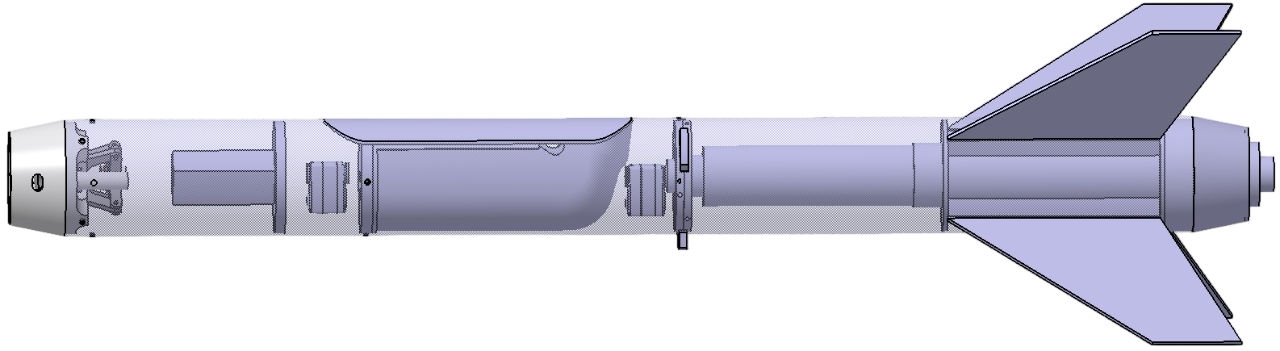
\includegraphics[width=\textwidth]{figures/catia_alpha.png}};
        
        \node (retreint_lbl)   at (+8.00, +2.5) {\textbf{Retreint}};
        \node (bloc_propu_lbl) at (+4.30, +2.3) {\textbf{Bloc propulsion}};
        \node (propu_lbl)      at (+2.00, +1.5) {\textbf{Pro54-5G}};
        \node (aileron_lbl)    at (+2.00, -1.5) {\textbf{Ailerons (x4)}};
        \node (af_lbl)         at (+0.00, +2.3) {\textbf{Aérofreins (x3)}};
        \node (bloc_para_lbl)  at (-2.00, +1.5) {\textbf{Bloc parachute}};
        \node (bloc_elec_lbl)  at (-6.00, +2.3) {\textbf{Bloc électroniques}};
        \node (bloc_sepa_lbl)  at (-6.00, -1.5) {\textbf{Bloc séparation}};

        \node (bloc_propu_box) at (+5.10, 0.00) [minimum width=35mm, minimum height=18mm, rectangle, line width=2, draw=red] {};
        
        \draw[red, ->, line width=1.5] (retreint_lbl.south)   -- (+7.20, +0.60);
        \draw[red, ->, line width=1.5] (bloc_propu_lbl.south) -- (bloc_propu_box.140);
        \draw[red, ->, line width=1.5] (propu_lbl.south)      -- (+2.20, +0.00);
        \draw[red, ->, line width=1.5] (aileron_lbl.east)     -- (+6.50, -1.50);
        \draw[red, ->, line width=1.5] (af_lbl.south)         -- (+0.30, +0.60);
        \draw[red, ->, line width=1.5] (bloc_para_lbl.south)  -- (-2.00, +0.00);
        \draw[red, ->, line width=1.5] (bloc_elec_lbl.south)  -- (-5.30, +0.00);
        \draw[red, ->, line width=1.5] (bloc_sepa_lbl.north)  -- (-7.30, +0.00);

    \end{tikzpicture}
    \caption{Vue du premier étage sur \acrshort{CATIA}}
    \label{fig:sp02_s1_ork}
\end{figure}



\subsubsection{Flèche}
\label{subsubsec:premier_etage}
À la suite de la conception, nous avons pu réaliser les tubes de la strcuture porteuse de la fusée. Nous avons procédé à un test de flèche sur les tubes afin de nous assurer de la bonne tenue mécanique de ces derniers.\\
Pour le tube du premier étage, nous avons encastré le tube comme si tenu par le propulseur et réalisé les tests comme au C'Space. 
\begin{table}[h!]
\centering
\begin{tabular}{|c|c|c|}
\hline
Positionnement & Flèche statique & Flèche dynamique \\ \hline
Patins à 0° & 0mm & 1mm \\ \hline
Patins à 90° & 0mm & 1,5mm \\ \hline
Patins à 180° & 0mm & 1mm \\ \hline
Patins à 270° & 0mm & 2mm \\ \hline
\end{tabular}
\end{table}



\subsubsection{Fabrication et collage du bloc propulsion avec ailerons}
Le bloc propulsion de SP-02 reprend la même architecture générale que celle définie pour SP-01, à savoir quatre ailerons en fibre de verre fixés sur un tube porte-moteur intégré dans le fuselage. Le rétreint arrière est de nouveau utilisé pour optimiser la réduction de traînée, mais le système de maintien du propulseur évolue : la vis latérale utilisée sur SP-01 est remplacée par une bague filetée venant se visser à l’arrière du tube porte-moteur, assurant un appui axial direct sur le propulseur. Cette modification permet de conserver la même géométrie extérieure tout en simplifiant la transmission des efforts axiaux et en maintenant la compatibilité avec le format moteur retenu.\\
\begin{figure}[h]
    \centering
    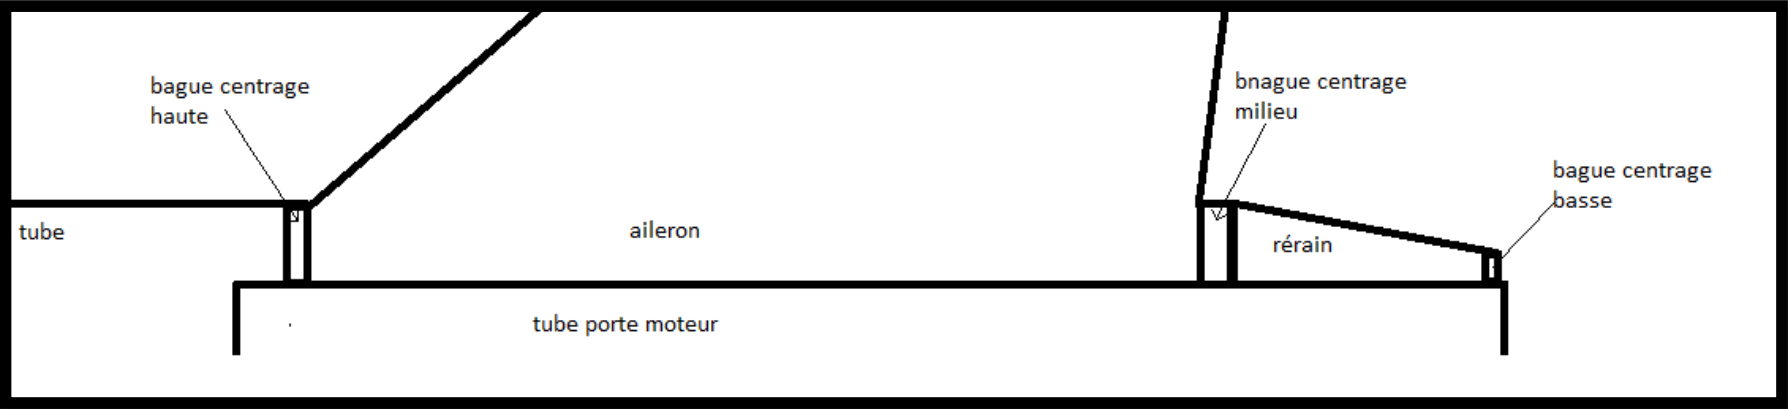
\includegraphics[width=\textwidth]{figures/schema1_SP-01.PNG}
    \caption{Procédé de collage ailerons/tube porte-moteur}
    \label{fig:collage_aileronsSP01}
\end{figure}
Le tube porte-moteur de SP-02, déjà fabriqué, reprend exactement le même principe de géométrie et de construction que celui utilisé pour SP-01. Réalisé à partir d’un moulage sur casing Pro-54, il possède un diamètre identique au standard attendu et conserve une longueur réduite par rapport au casing d’origine afin d’optimiser la masse tout en maintenant une rigidité suffisante pour supporter l’ensemble du bloc propulsion. Les ailerons seront ensuite collés à la résine époxy sur ce tube déjà réalisé, ainsi que sur les deux bagues de centrage, de manière à reproduire fidèlement la configuration mécanique utilisée précédemment et à assurer une continuité dans l’intégration structurelle du bloc propulsion.\\
\begin{figure}[h]
    \centering
    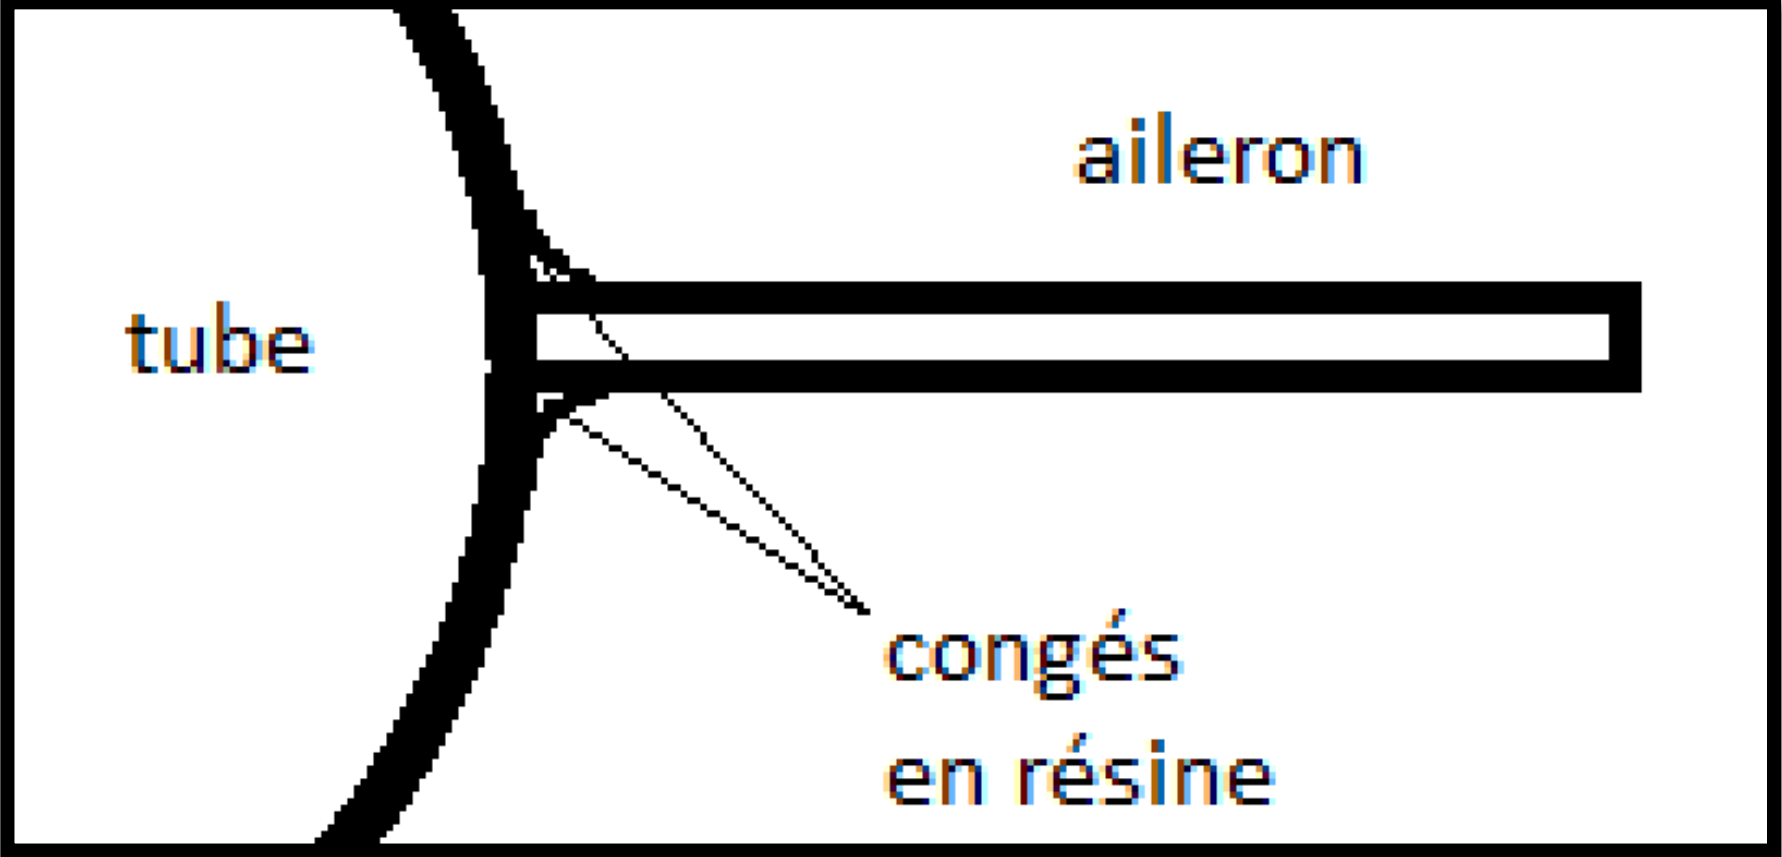
\includegraphics[width=\textwidth]{figures/schema3_SP-01.PNG}
    \caption{Procédé de collage ailerons/structure avec congés en résine}
    \label{fig:collage2_aileronsSP01}
\end{figure}
Enfin, SP-02 reprend également la logique de finition appliquée sur SP-01 : des perçages seront réalisés en amont et en aval des ailerons afin de garantir une diffusion homogène de la résine dans la zone d’assemblage, et des congés en résine seront appliqués sur les jonctions extérieures pour assurer une transition aérodynamique lisse. Cette étape permet également de fermer proprement les points d’injection tout en assurant une finition aérodynamique cohérente avec le modèle précédent.\\